\chapter{Architecture}

\section{Vue d'ensemble}

La vue d'ensemble de l'architecture est présentée dans la~\autoref{fig:architecture}.
Il y 6 machines virtuelles (VM) au total dont 5 conçues depuis Nuvla et
1 VM permanente déployée sur le cloud \cloudInstance{ifb-prabi-girofle}.

\begin{figure}[htp]
    \centering
    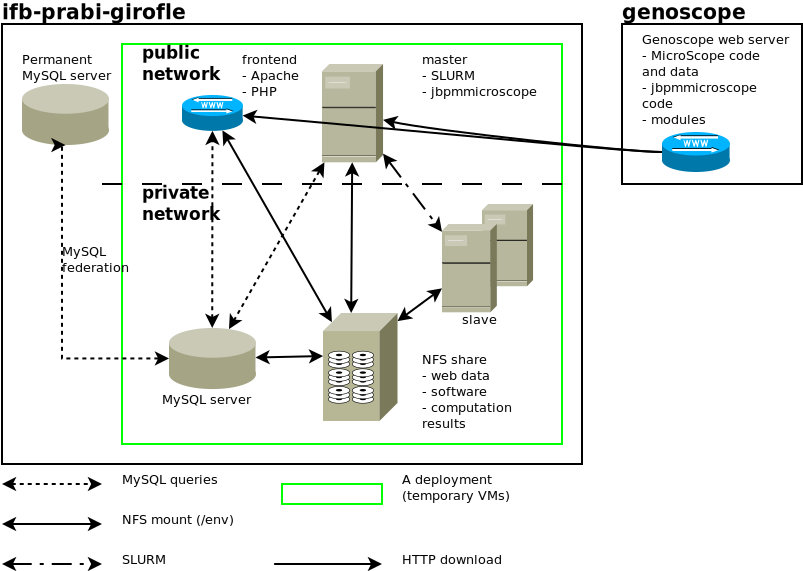
\includegraphics[width=\linewidth]{../Logical_Architecture}
    \caption{Schéma de l'architecture de MicroCloud.}
    \label{fig:architecture}
\end{figure}

Un des buts est de mimer ce qui est fait au Genoscope
c'est-à-dire que:
\begin{enumerate}
    \item Les différents composants (serveur web, serveur de BD) tournent sur des machines séparées.
    \item Les calculs tournent sur des machines séparées: l'architecture contient donc un cluster (basé sur SLURM).
\end{enumerate}
Une des seules différences est que le serveur \component{jbpmmicroscope} tourne
sur la machine frontale du cluster.

Il y a 2 serveurs de bases de données dans MicroCloud:
\begin{itemize}
    \item Un serveur MySQL installé via Docker dans la VM MySQL.
    \item Un serveur MySQL sur la VM permanente.
\end{itemize}

\section {Installation et déploiement des VM}

Le code des VM Nuvla est dans le dépôt biosphere-microcloud (\url{https://github.com/IFB-ElixirFr/biosphere-microcloud/}).
Il y a un dossier par VM et un fichier \filename{README.md} dans chaque dossier qui explique des détails.
Les principes du déploiement sont décrits sur le wiki du projet (voir la page
\href{https://intranet.genoscope.cns.fr/agc/redmine/projects/microcloud/wiki/Principes_de_fonctionnement_du_cloud_IFB}
{[[Principes de fonctionnement du cloud IFB]]}
en particulier la section
\href{https://intranet.genoscope.cns.fr/agc/redmine/projects/microcloud/wiki/Principes_de_fonctionnement_du_cloud_IFB#Utilisation-de-deacutepocircts-git-pour-le-code}
{[[Principes de fonctionnement du cloud IFB\#Utilisation-de-deacutepocircts-git-pour-le-code]]}
).

Les sections suivantes présentent quelques détails sur les VM:
\begin{itemize}
    \item frontend voir section \ref{frontend}
    \item mysql voir section \ref{mysql}
    \item VM permanente voir section \ref{VMpermanente}
    \item master et slave voir section \ref{master&slave}
    \item nfsserver voir section \ref{nfsserver}
\end{itemize}

\subsection {VM frontend}\label{frontend}

\todo[inline]{Ajouter une section sur les scripts côté serveur qui permettent d'installer le logiciel.}

La VM frontend permet de déployer la partie web de la plateforme MicroScope.
L'image de base est une image CentOS 7.

Le code est dans le dossier frontend (voir \url{https://github.com/IFB-ElixirFr/biosphere-microcloud/tree/master/frontend/}).
Le composant slipstream est dans le dossier frontend (voir \url{https://nuv.la/module/ifb/devzone/MicroCloud/frontend/}).

Lors du déploiement de la VM le code web est copié dans le répertoire \textbf{/var/www/html/} de la VM.

La VM frontend utilise un client mariaDB (et non pas MySQL du fait de conflits existants entre le dépôt remi-php71 installé et le dépôt IUS qui fournit le client MySQL).



\begin{mycolorbox}
    Si le message d'erreur \textbf{256} s'affiche, cela signifie simplement qu'il n'y a pas d'organisme en base.
    De ce fait, la plupart des onglets ainsi que le formulaire d'authentification sont inaccessibles.
    Ceci ne doit pas arriver si le déploiement se passe bien car on on copie les données d'un organisme.
\end{mycolorbox}

\subsection {VM mysql}\label{mysql}

Le code est dans le dossier mysql voir \url{https://github.com/IFB-ElixirFr/biosphere-microcloud/tree/master/mysql/}.
Le composant slipstream est dans le dossier mysql voir \url{https://nuv.la/module/ifb/devzone/MicroCloud/mysql/}.

L'image de base est une image CentOS 7. La VM mysql possède un serveur MySQL installé via Docker sur lequel on retrouve les bases de données pkgdb, GO\_CPD, GO\_Conf, GO\_RES, PUB\_CPD, REFSEQDB, JBPMmicroscope et PRESTATIONDB. Les tables nécessaires à l'installation de MicroScope sont également listées dans le wiki : \url{https://intranet.genoscope.cns.fr/agc/redmine/projects/microcloud/wiki/Tables_necessaires_a_installation}.

Pour se connecter à la VM mysql, il faut passer par le frontend :
\begin{lstlisting}[style=bash]
$ ssh -A centos@${IP_mysql} -J centos@${IP_frontend}
\end{lstlisting}

Si le serveur ne répond pas, il faut aller voir si le docker n'a pas planté (cela arrive pour des requêtes SQL trop gourmandes en RAM).
Pour relancer le docker :
\begin{lstlisting}[style=bash]
$ sudo su
$ docker ps -a
$ docker start ${ID_container}
\end{lstlisting}

\subsection {VM permanente}\label{VMpermanente}

C'est une VM OpenStack (\textbf{umr5558-microcloud.univ-lyon1.fr}) du cloud \cloudInstance{ifb-prabi-girofle} disposant de 200 Go de stockage et 8 Go de RAM (elle est actuellement sous-dimensionnée par rapport à nos besoins). La machine a été installée avec Sylvain Bonneval. L'image de base est une image Debian 9.8.

La machine permanente n'est accessible depuis l'extérieur qu'en SSH donc nous ne pouvons pas y accéder en MySQL (port 3306) depuis un autre cloud.

La procédure d'installation est dans le fichier \textbf{Installation.md} du répertoire \textbf{/root}. La VM permanente sert au stockage des données des banques. Nous avons utilisé \textbf{rsync} pour l'import des données dans le serveur MySQL.

Logiciels installés : serveur MySQL, rsync, phpMyAdmin (installé mais non configuré). 

Pour se connecter : 
\begin{lstlisting}[style=bash]
$ ssh root@134.214.33.214
\end{lstlisting}

Sur le serveur MySQL, il y a les schémas des bases DB et une partie des données de la base pour les tests (nous avons testés les onglets \textbf{Genome Browser}, \textbf{Identical Gene Names}) :
\begin{itemize}
    \item les bases ANTISMASHDB, CARDDB, COGDB, EGGNOGDB, ENZYMEDB, ESSDB, FIGFAMDB, INTERPRODATADB, KEGGDB, RHEADB, TAXONOMYDB, TIGRFAMDB, UNIFIREDB, UNIPROTKBDB, VIRULENCEDB, microcyc, DBWorkflow
    \item les données (en partie) de la base UNIPROTKBDB pour les tests
    \item les données de DBWORKFLOW
    \item les données de l'organisme \theOrg{} (taxon id \theTaxID{}) dans la base TAXONOMYDB
\end{itemize}

Le script \script{microscopeDBschema.py} du module MicroCloud a été utilisé pour créer les schémas.

Pour se connecter au serveur MySQL :
\begin{lstlisting}[style=bash]
$ mysql -p{MOT_DE_PASSE_SERVEUR_MYSQL_VM_PERMANENTE}
\end{lstlisting}

Les mots de passe (serveur MySQL et phpMyAdmin) sont stockés dans le répertoire \textbf{/root} de la VM.

Pour copier les données, mieux vaut utiliser rsync et copier les données dans le répertoire \textbf{/var/lib/mysql-files/} de la VM permanente avant insertion en base.

\begin{lstlisting}[style=bash]
$ LOAD DATA INFILE '/var/lib/mysql-files/$file.DB' INTO TABLE $table;
\end{lstlisting}

\subsection{VM master et VM slave(s)} \label{master&slave}

\todo[inline]{Ajouter les notes sur jbpmmicroscope ici ? Notes sur conda et l'installation des modules ?}

Le code d'installation de ces VM est dans le dépôt de biosphere-commons : \url{https://github.com/IFB-ElixirFr/biosphere-commons}.
L'image de base est une image Ubuntu 18. Le code slipstream est basé sur les travaux de Jonathan Lorenzo et Bryan Brancotte. 

Les composants master et slave ont été copiés depuis l'appliance Slurm\_Cluster\_ubuntu18 voir \url{https://nuv.la/module/ifb/devzone/jlorenzo/cluster/Slurm_Cluster_ubuntu18}.

Concernant la VM master, le code est dans le dossier master; voir
\url{https://github.com/IFB-ElixirFr/biosphere-microcloud/tree/master/master/}.
Le code du composant slipstream est dans le dossier master voir; \url{https://nuv.la/module/ifb/devzone/MicroCloud/master/}.

Pour la VM slave, voir les dossiers correspondants.\newline

Nous avons installé le moteur de workflow jBPM couplé avec un cluster SLURM sur la VM master. L'ordonnancement des wokflows est ensuite géré à l'aide du cluster SLURM. La VM master étant considérée comme la machine maître et les VM slaves comme noeuds de calcul.

Le serveur d'application Tomcat est installé (version tomcat-9.0.31 : \url{http://mirrors.ircam.fr/pub/apache/tomcat/tomcat-9/v9.0.31/bin/apache-tomcat-9.0.31.tar.gz}).
Il est utilisé comme serveur par jBPM (pour accéder à Tomcat : http://\$IP\_master).

Nous avons également eu besoin d'installer Pegasus-mpi-cluster (version 4.9.2 : \url{https://github.com/pegasus-isi/pegasus/archive/4.9.2.zip}) en complément de jBPM. Lors de l'installation de pegasus-mpi-cluster, la librairie libnuma a posé problème mais celle-ci n'est pas nécessaire pour les architectures non NUMA (voir \url{https://github.com/IFB-ElixirFr/biosphere-microcloud/blob/master/master/04_deployment.sh}).

Chaque workflow fait appel à différents modules qu'il faut installer au préalable sur la VM master. Le script \url{https://github.com/IFB-ElixirFr/biosphere-microcloud/blob/master/master/import_modules.sh} permet d'importer les archives des différents modules nécessaires au fonctionnement des workflows (WF DIRECTON principalement).
Le lancement des workflows se fait à l'aide du module bagsub lui-même lancé par jBPM. Nous avons fait quelques modifications du module bagsub afin qu'il puisse être utilisé dans l'environnement fourni par la VM master. Le script \script{import\_modules.sh} modifie le module bagsub, en supprimant l'option ulimit qui ne fonctionne pas en Dash, et, en ajoutant le paramètre MCA btl\_tcp\_if\_exclude pour exclure les interfaces réseaux docker0 et lo qui peuvent engendrer des conflits lors du lancement de jobs SLURM.


\subsection{VM nfsserver} \label{nfsserver}

Le composant nfsserver a été créé en s'inspirant du travail de Stéphane Delmotte.
Il permet de fournir un dossier partagé entre les différentes VM.

L'image de base est une image CentOS 7.
Le code est dans le dossier nfsserver voir  \url{https://github.com/IFB-ElixirFr/biosphere-microcloud/tree/master/nfsserver/}.
Le composant slipstream est dans le dossier nfsserver voir
\url{https://nuv.la/module/ifb/devzone/MicroCloud/nfsserver/}.

Le répertoire \path{/var/nfsshare} du serveur NFS est monté dans le répertoire \path{/env}
des VM frontend, backend, master et slave(s).
Le répertoire \textbf{/env} se veut similaire au répertoire de même nom sur le cluster etna. 
Les fonctions permettant la création du répertoire partagé sont dans le fichier \url{https://github.com/IFB-ElixirFr/biosphere-microcloud/blob/master/lib.sh}.

